\section{Evaluation}
\label{Sec-Evaluation}

In this section, we discuss results on a Sun SPARC T5240, which contains two UltraSPARC T2 Plus chips with 8 cores each, running at 1.165 GHz. Each core has 8 hardware strands, for a total of 64 hardware threads per chip. A core has a 8KB L1 data cache and shares an 4MB L2 data cache with the other cores on a chip. Each experiment was performed five times and we report the median. Variance was very low for all experiments. Each test was run for ten seconds to measure throughput. We used the same benchmark as flat combining~\cite{Hendler2010}. A thread randomly flips a coin with  probability $p$ to be an \texttt{PQ::add()} and $1-p$ to be a \texttt{PQ::removeMin()}. We started a run after inserting 2000 elements in the priority queue for stable state results. 

Our priority queue algorithm (\emph{pqe}) uses combining and elimination, and leverages the parallelism of \texttt{PQ::add()}. We performed experiments to compare against previous priority queues using combining methods, such as flat combining skiplist (\emph{fcskiplist}) and flat combining pairing heap (\emph{fcpairheap}). We also compared against previous priority queues using skiplists with parallel operations, such as a lock free skiplist (\emph{lfskiplist}) and a lazy skiplist (\emph{lazyskiplist}). The flat combining methods are very fast at performing \texttt{PQ::removeMin()} operations, which then get combined and executed together. However, performing the \texttt{PQ::add()} operations sequentially is a bottleneck for these methods. Conversely, the \emph{lfskiplist} and \emph{lazyskiplist} algorithms are very fast at performing the parallel adds, but get significantly slowed down by having \texttt{PQ::removeMin()} operations in the mix, due to the synchronization overhead involved. Our \emph{pqe} design tries to address these limitations through our \emph{dual} (sequential and parallel parts), \emph{adaptive} implementation that can be beneficial in the different scenarios. 

\begin{figure}[htb]
\centering
\begin{minipage}[b]{.495\textwidth}
	\centering
  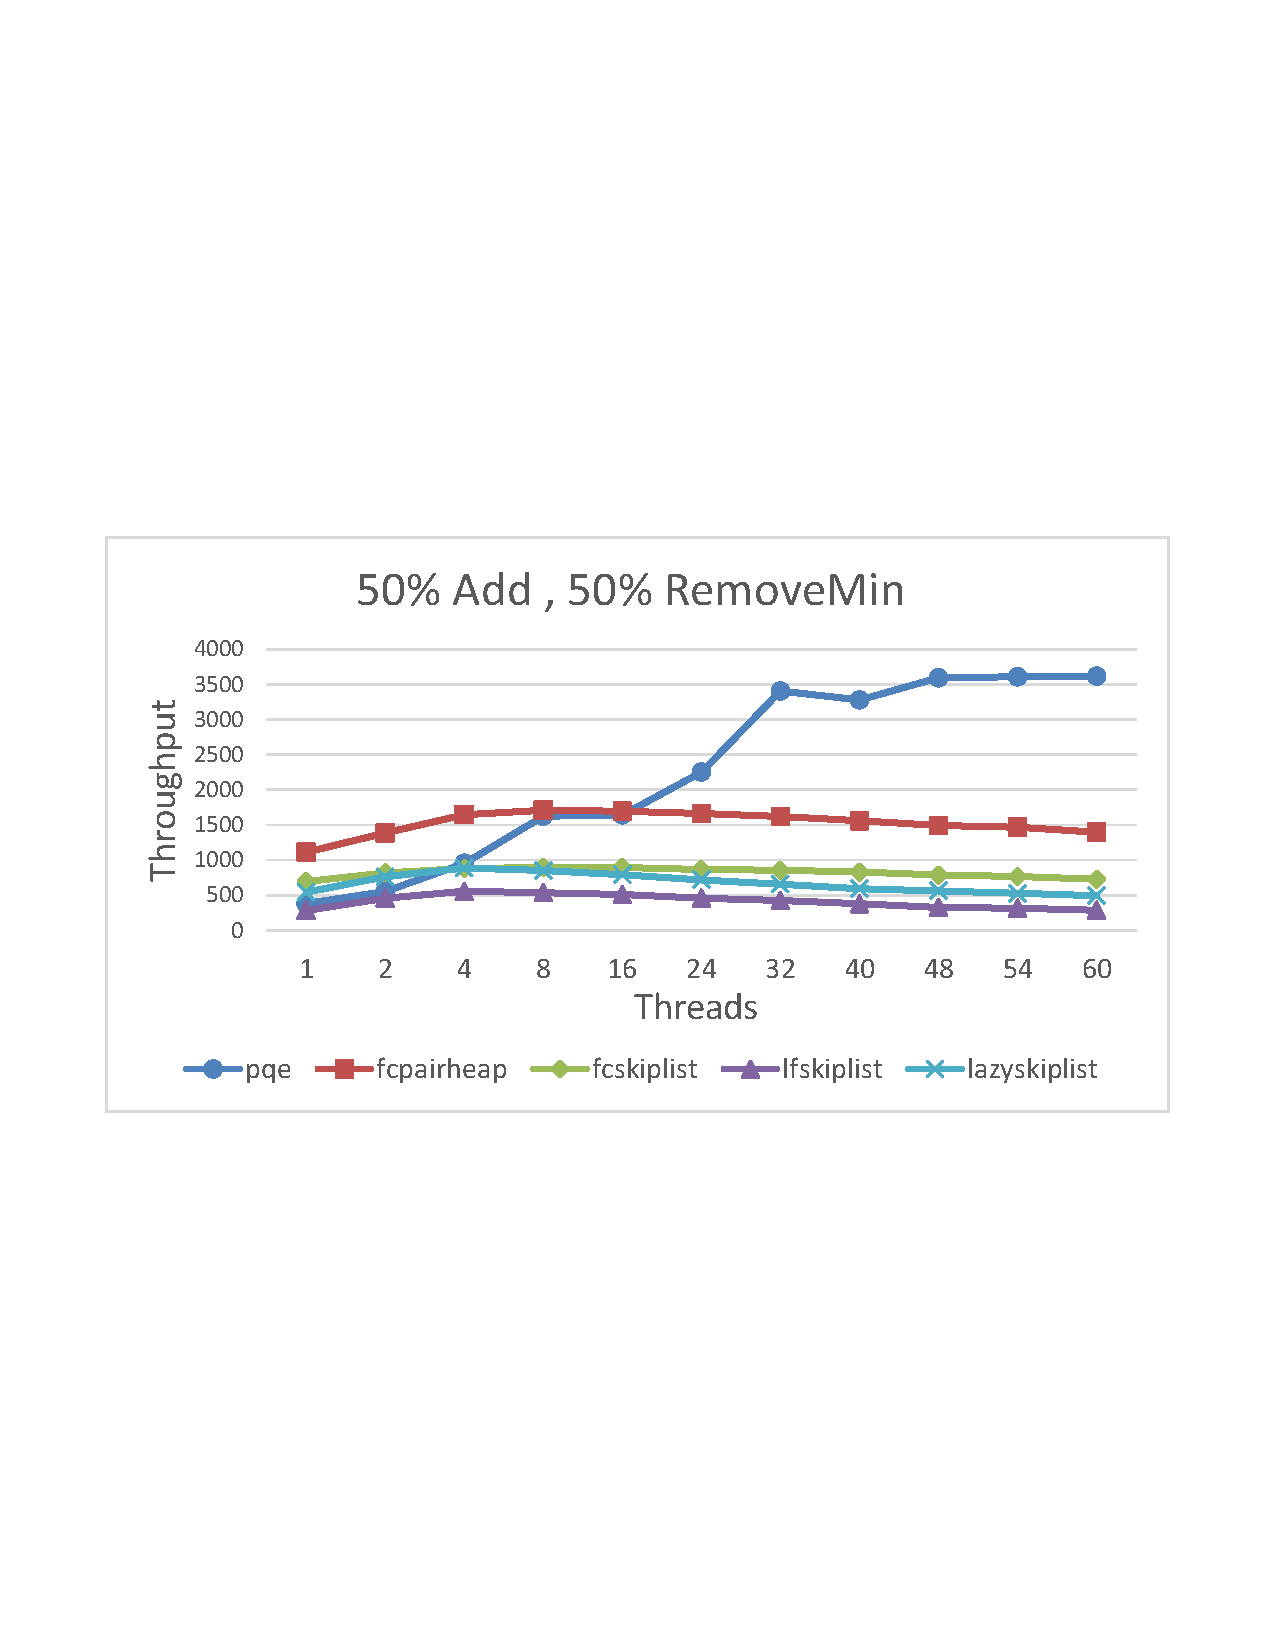
\includegraphics[width=\linewidth]{img/sparc-50-50.pdf}
\caption{Priority queue performance with 50\% \texttt{add()}s, 50\% \texttt{removeMin()}s.}
\label{fig:sparc_50}
\end{minipage}%
\hfill%
\begin{minipage}[b]{.495\textwidth}
	\centering
  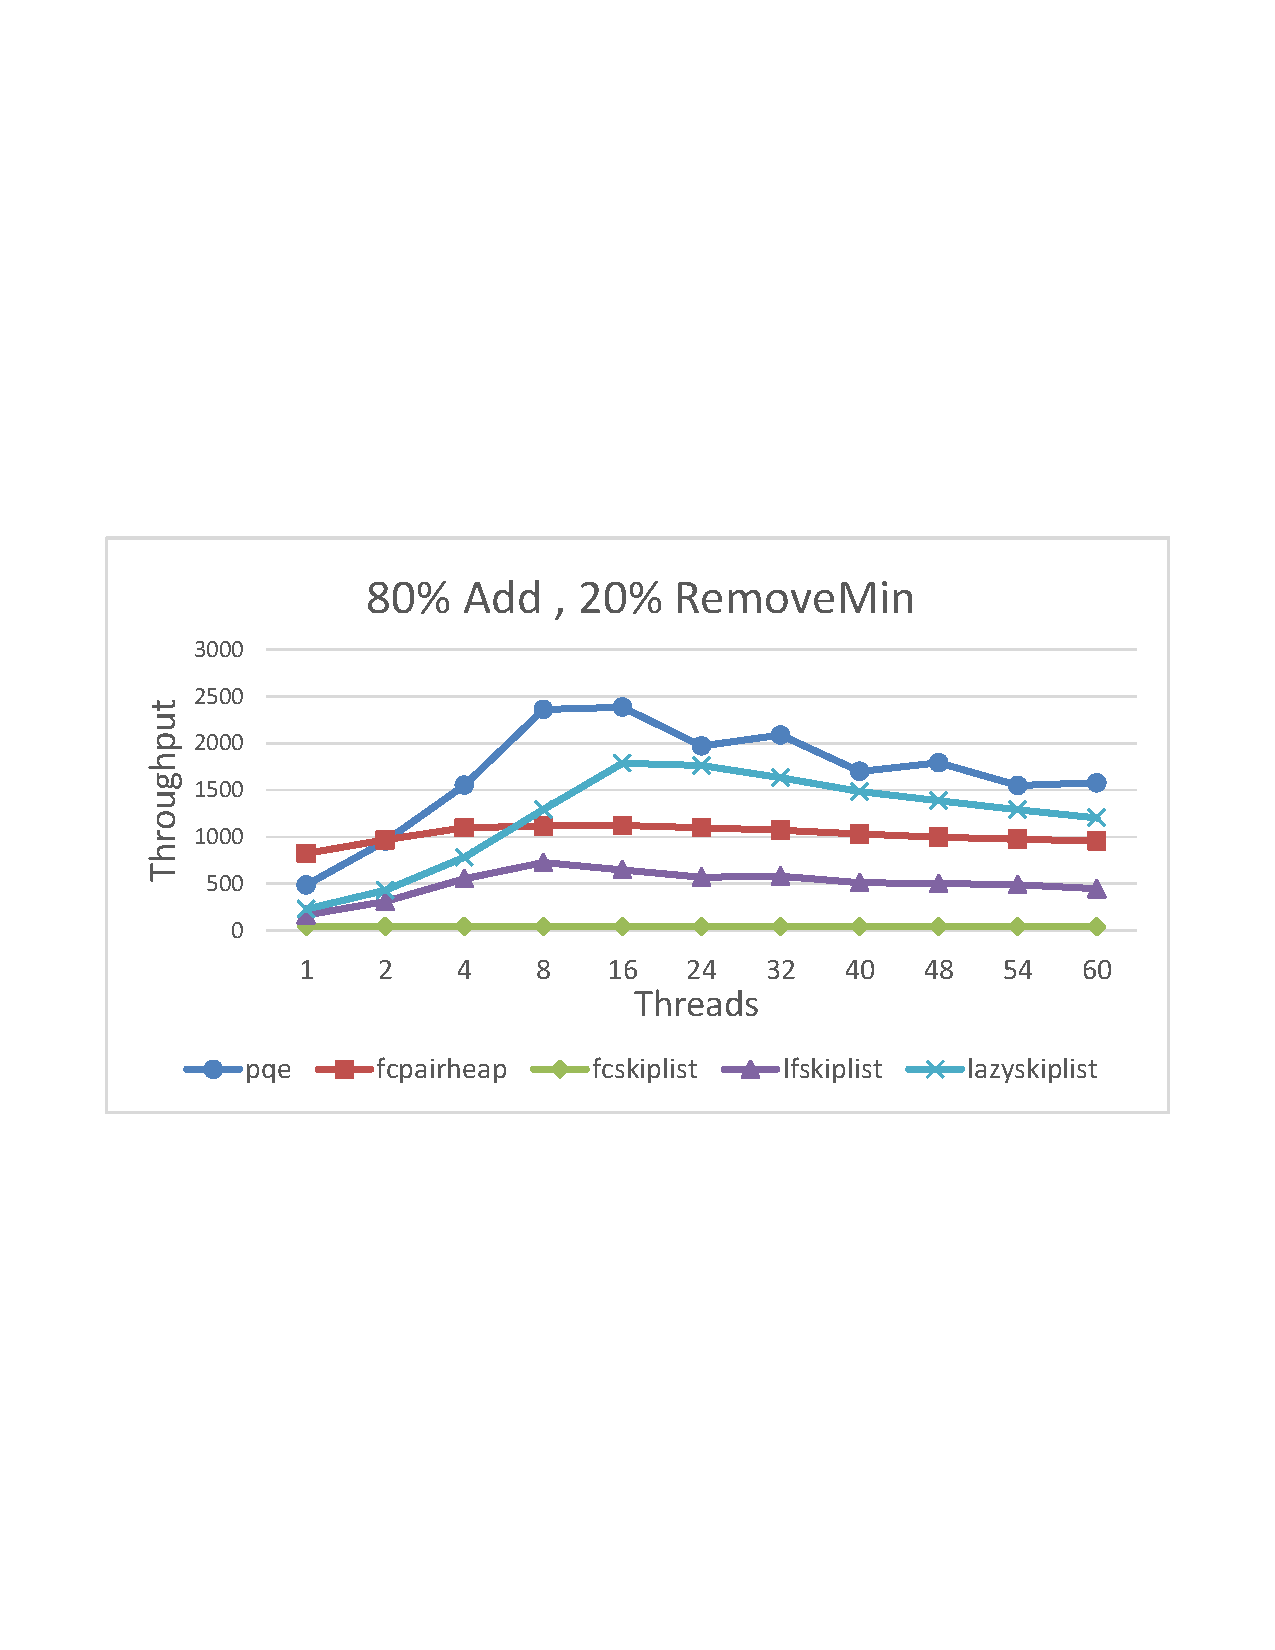
\includegraphics[width=\linewidth]{img/sparc-80-20.pdf}
\caption{Priority queue performance with 80\% \texttt{add()}s, 20\% \texttt{removeMin()}s.}
\label{fig:sparc_80}
\end{minipage}%
\end{figure}

\begin{figure}[htb]
\centering
\begin{minipage}[b]{.495\textwidth}
	\centering
  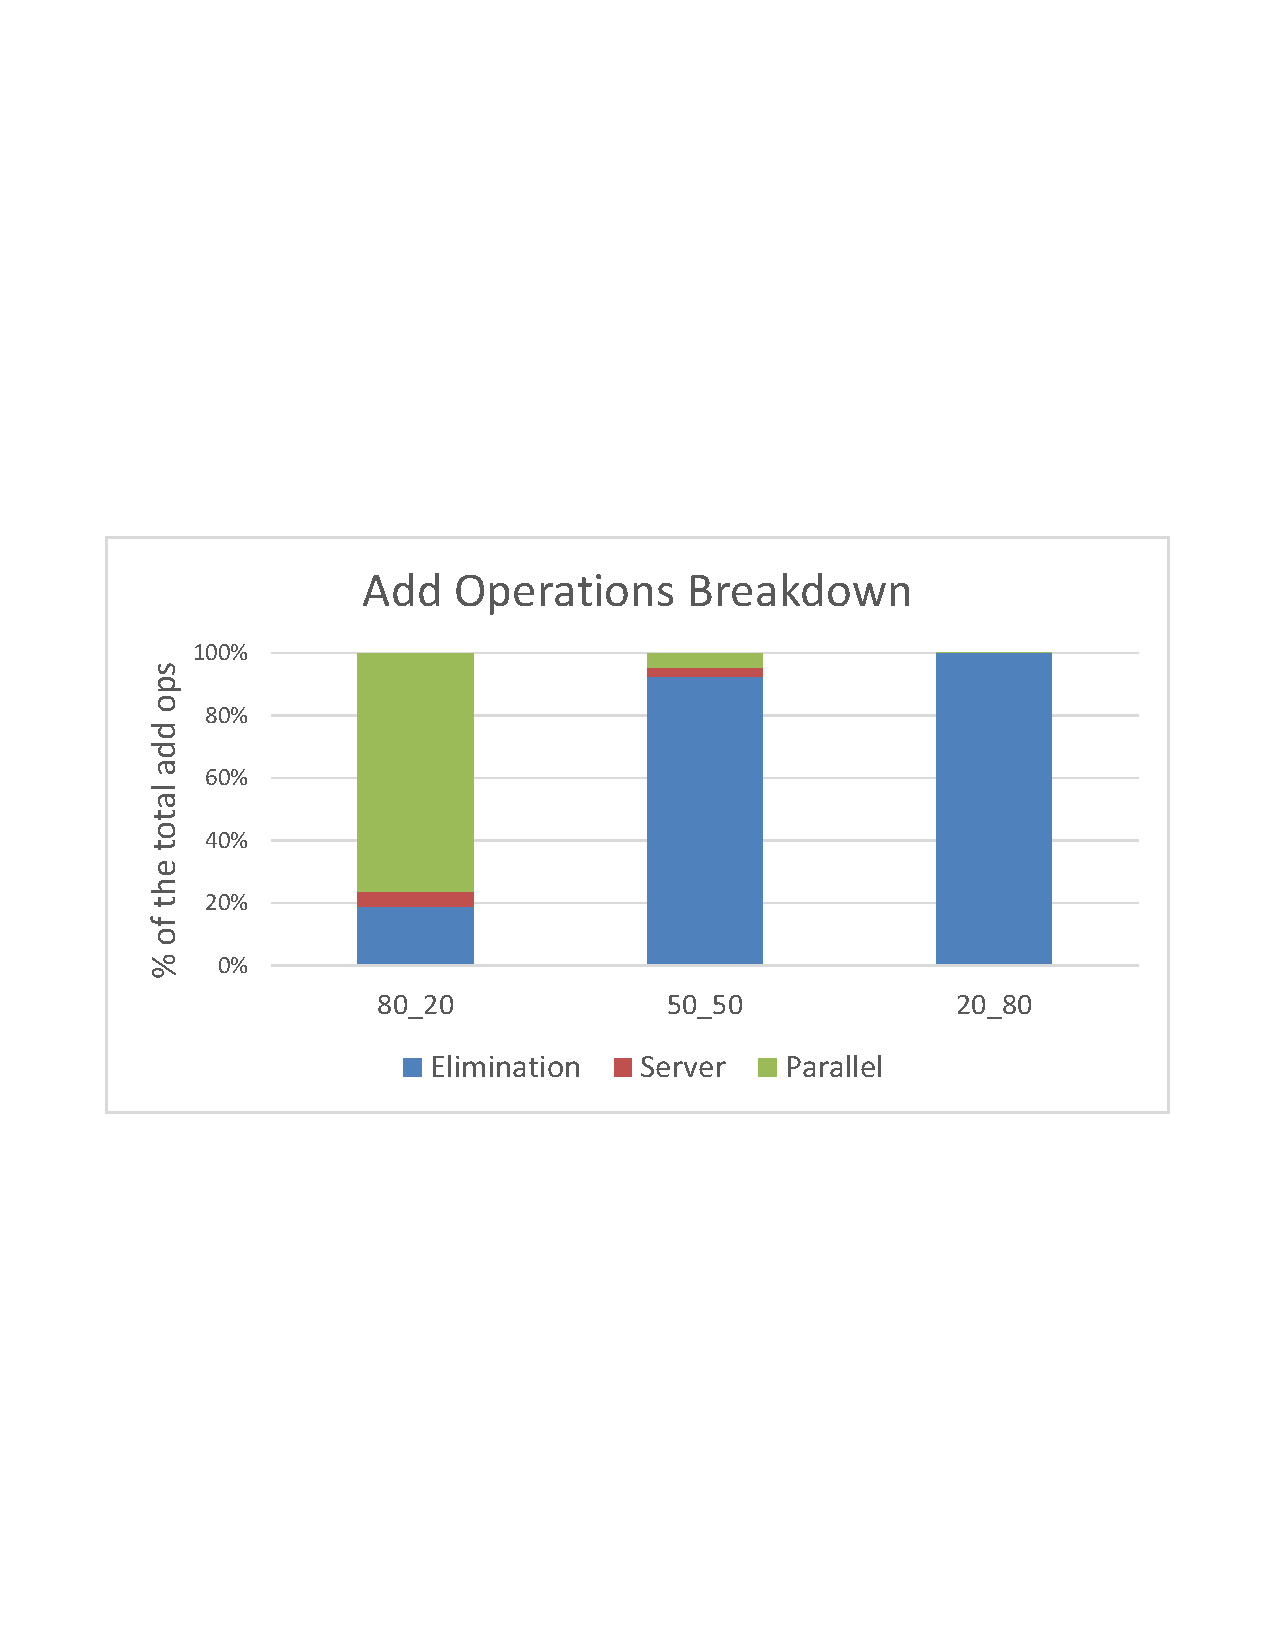
\includegraphics[width=\linewidth]{img/sparc-add-brk.pdf}
\caption{\texttt{add()} work breakdown.}
\label{fig:sparc_add}
\end{minipage}%
\hfill%
\begin{minipage}[b]{.495\textwidth}
	\centering
  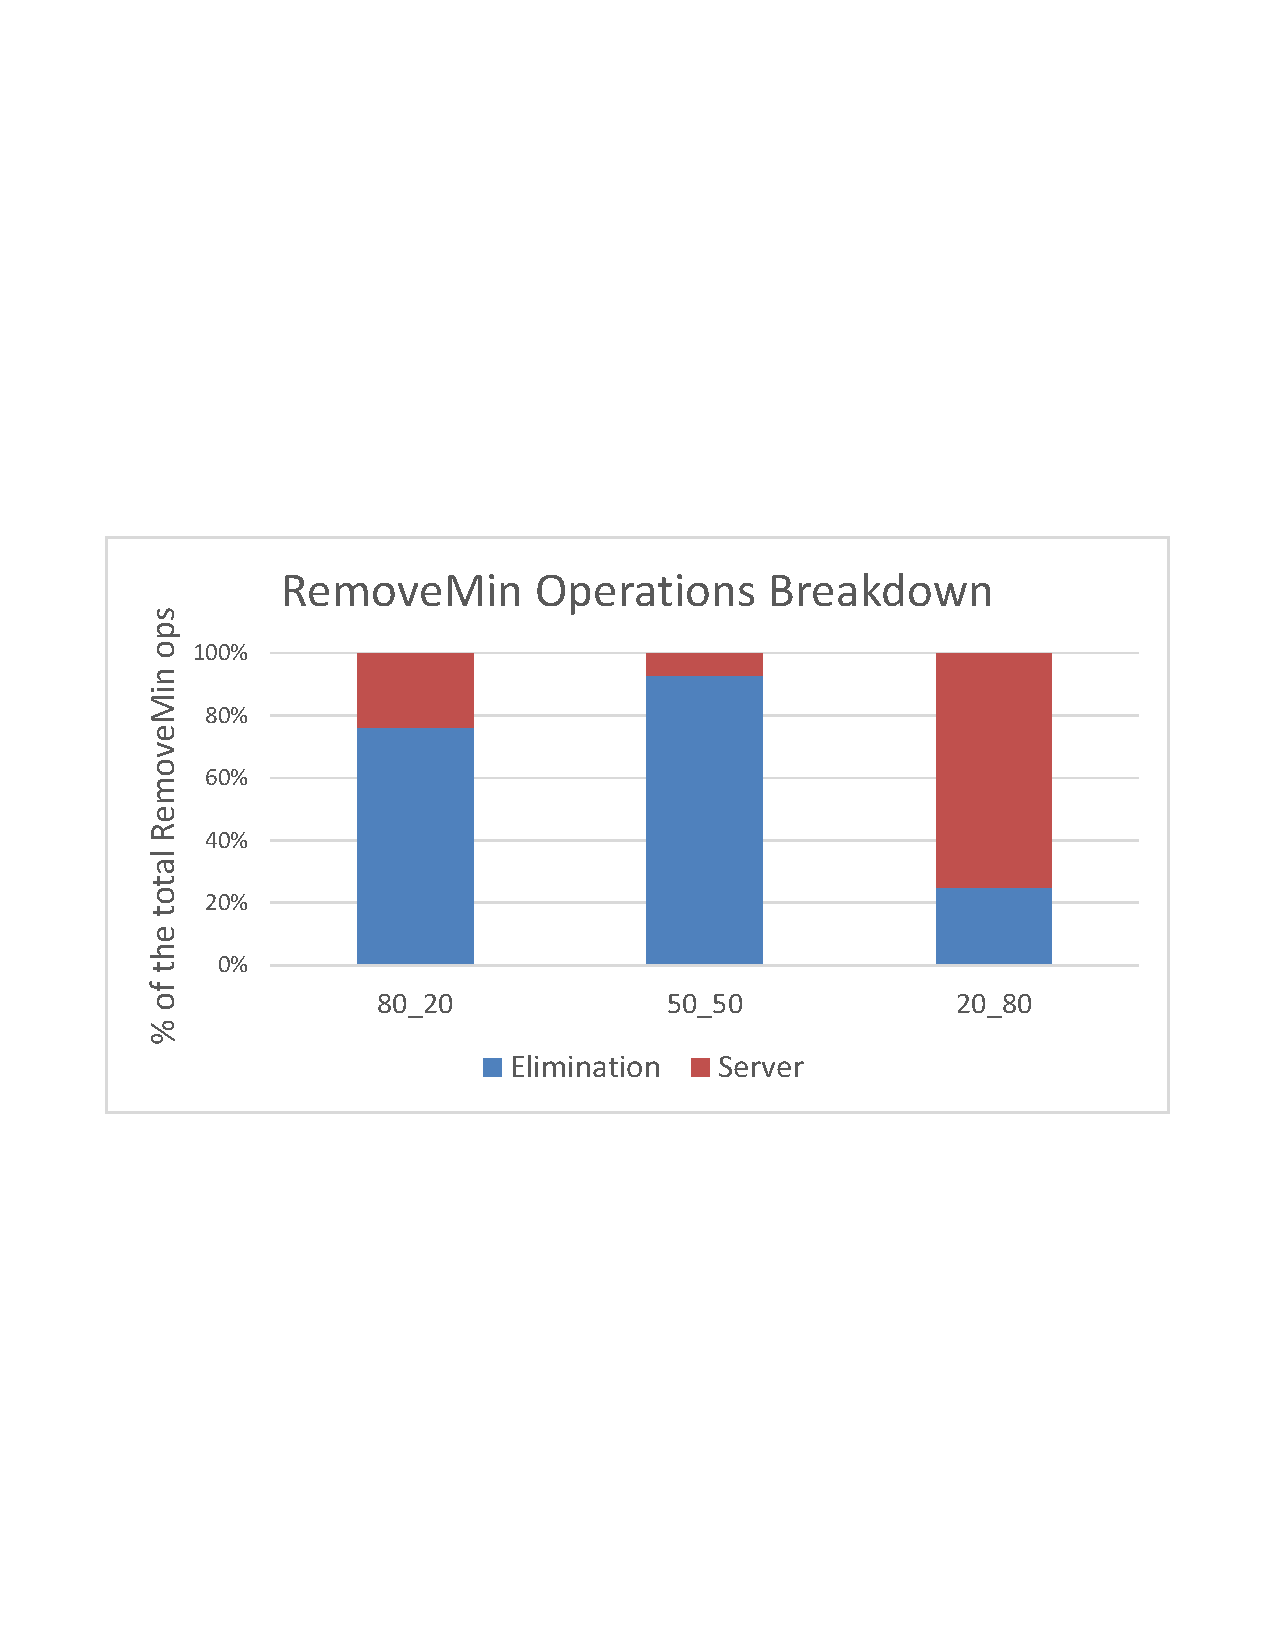
\includegraphics[width=\linewidth]{img/sparc-rem-brk.pdf}
\caption{\texttt{removeMin()} work breakdown.}
\label{fig:sparc_rem}
\end{minipage}%
\end{figure}

We considered different percentages of \texttt{PQ::add()} and \texttt{PQ::removeMin()} in our tests. When the operations are roughly the same number, \emph{pqe} can fully take advantage of both elimination and parallel adds, so it has peak performance. Figure~\ref{fig:sparc_50} shows how for $50\%$ \texttt{PQ::add()} and $50\%$ \texttt{PQ::removeMin()}, \emph{pqe} is much more scalable and can be up to 2.3 times faster than all other methods. When there are more \texttt{PQ::add()} than \texttt{PQ::removeMin()}, as in Figure~\ref{fig:sparc_80} with $80\%$ \texttt{PQ::add()} and $20\%$ \texttt{PQ::removeMin()}, \emph{pqe} behavior approaches the other methods, but it is still $70\%$ faster than all other methods at high thread counts. In this specific case there is only little potential for elimination, but having parallel insertion operations makes our algorithm outperform the flat combining methods. The \emph{lazyskiplist} algorithm also performs better than other methods, as it also takes advantage of parallel insertions. However, \emph{pqe} uses the limited elimination and the combining methods to reduce contention, making it faster than the \emph{lazyskiplist}. For more \texttt{PQ::removeMin()} operations than \texttt{PQ::add()} operations, the \emph{pqe}'s potential for elimination and parallel adds are both limited, thus other methods can be faster. \emph{Pqe} is designed for high contention scenarios, in which elimination and combining thrive. Therefore, it can incur a penalty at lower thread counts, where there is not enough contention to justify the overhead of the indirection caused by the elimination array and the server thread. 

To better understand when each of the optimizations used is more beneficial, we analyzed the breakdown of the \texttt{PQ::add()} and \texttt{PQ::removeMin()} operations for different \texttt{PQ::add()} percentages. When we have $80\%$ \texttt{PQ::add()}, most of them are likely to be inserted in parallel ($75\%$), with a smaller percentage being able to eliminate and an even smaller percentage being executed by the server, as shown in Fig.~\ref{fig:sparc_add}. In the same scenario, $75\%$ of \texttt{removeMin()} operations eliminate, while the rest gets execute by the server, as seen in Fig.~\ref{fig:sparc_rem}. For balanced workloads ($50\%-50\%$), most operations eliminate and a few \texttt{PQ::add()} operations are inserted in parallel. When the workload is dominated by \texttt{PQ::removeMin()}, most \texttt{PQ::add()} eliminate, but most \texttt{PQ::removeMin()} are still left to be executed by the server thread, thus introducing a sequential bottleneck. Eventually the priority queue would become empty, not being able to satisfy \texttt{PQ::removeMin()} requests with an actual value anymore. In this case, any \texttt{add()} operation can eliminate, allowing full parallelism. We do not present results for this case because it is an unlikely scenario that unrealistically favors elimination. 
